\documentclass[12pt]{article}
\usepackage{pdfpages}
\usepackage{eso-pic}
\usepackage{hyperref, url}
\usepackage{graphicx}
\graphicspath{{images/}}
\newcommand \tab[1][1cm]{\hspace*{#1}}

\begin{document}
\input{Titlu.tex}
\cleardoublepage

\section*{Lucrarea de laborator \#1}
\phantomsection

\section{Scopul lucrarii de laborator}
De a se invata utilizarea unui Version Control System si modul de setare a unui server.
\section{Obiective}
Studierea Version Control Systems (git).

\clearpage

\cleardoublepage

\section{Screenshoturi}
\textbf{Calculator \#1}\\
\\
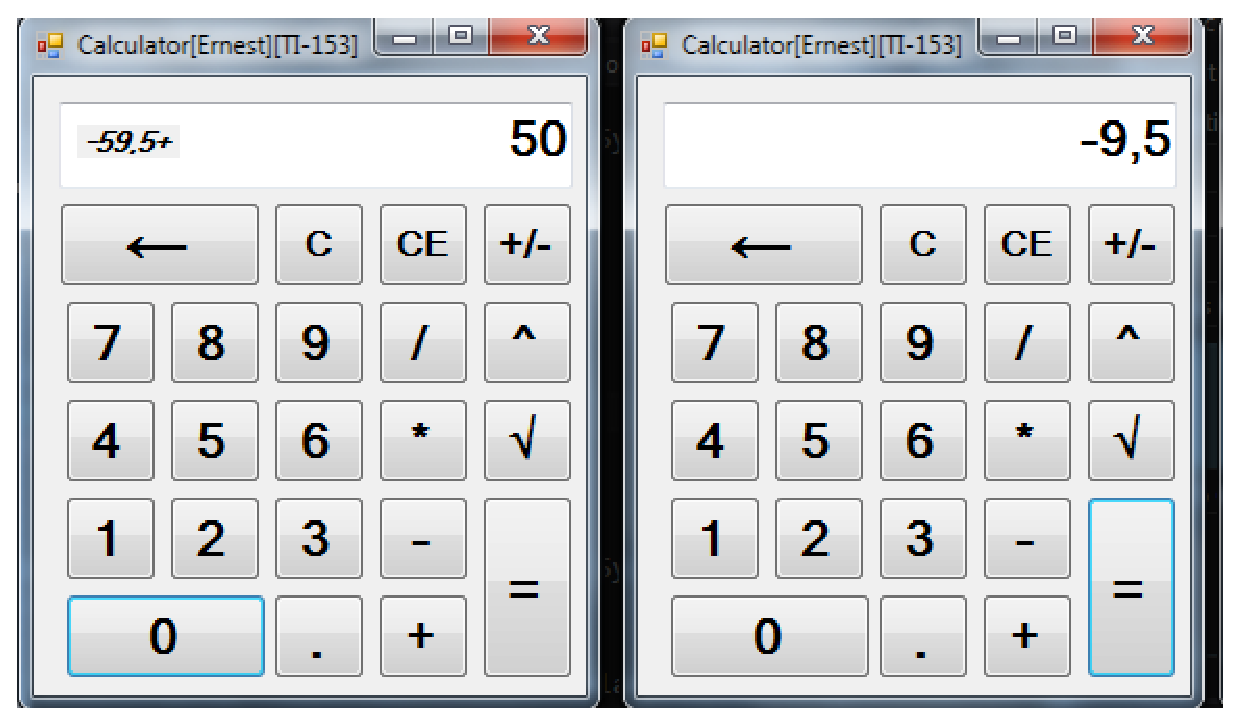
\includegraphics[width=\textwidth]{4.eps}\\
\\
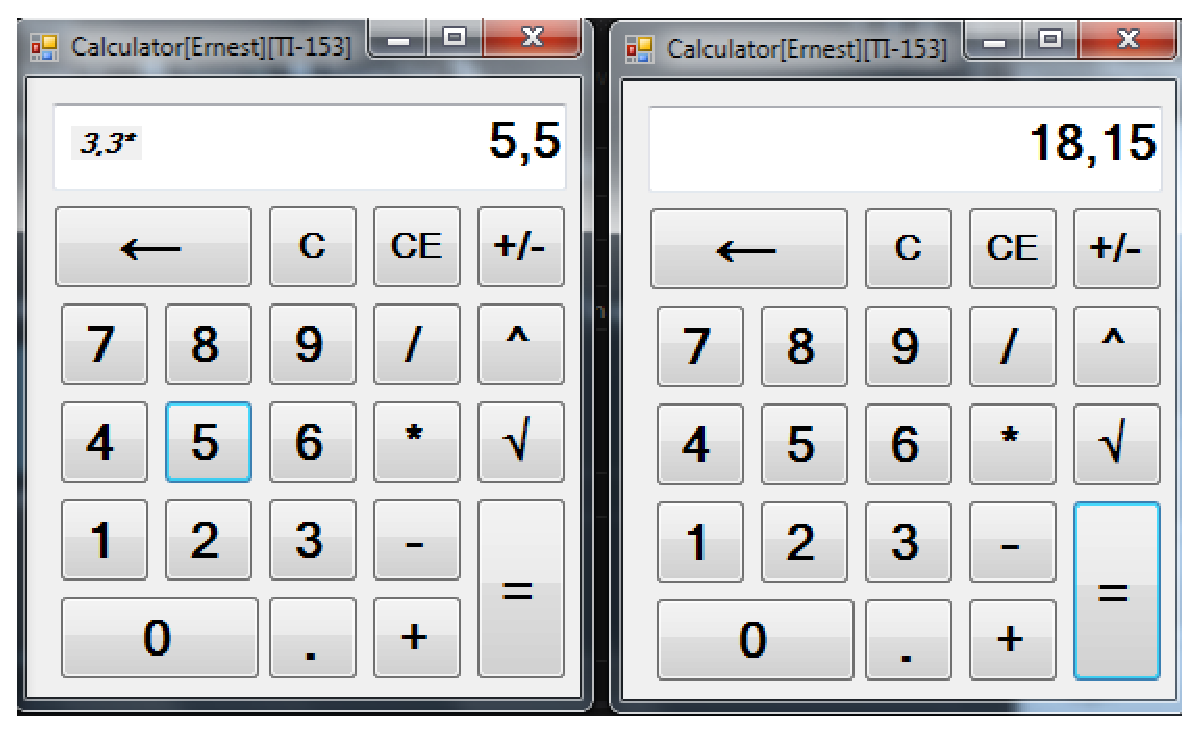
\includegraphics[width=\textwidth]{5.eps}\\
\clearpage
\textbf{Calculator \#2}\\
\\
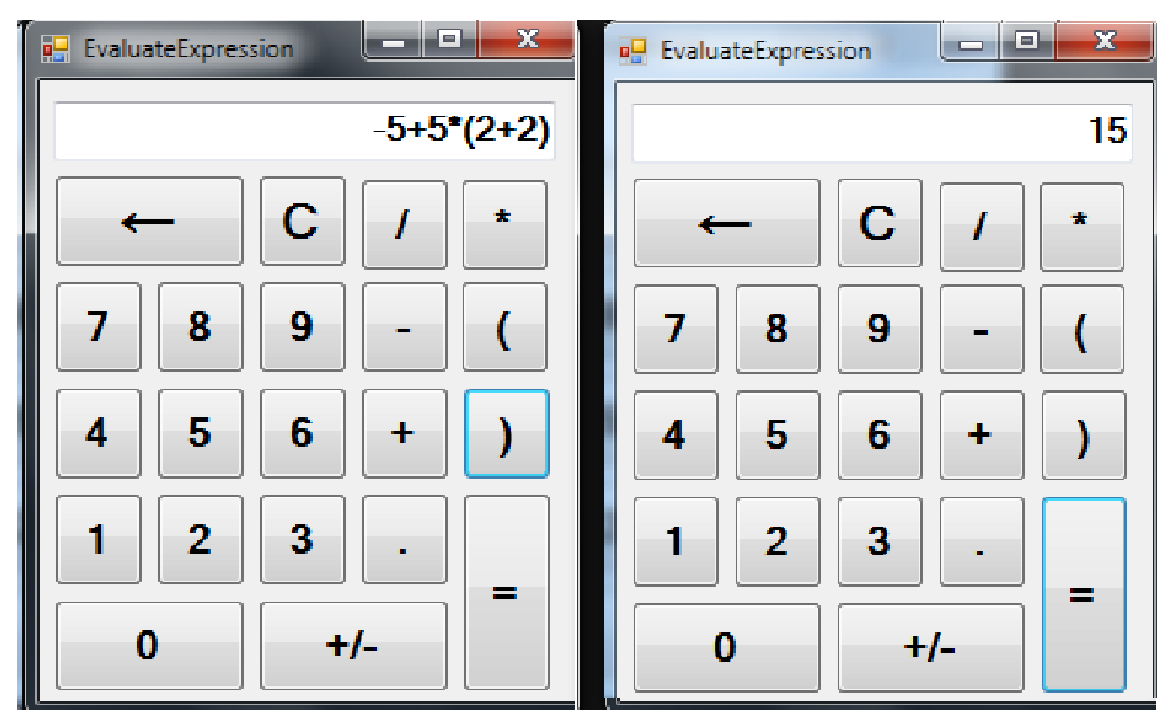
\includegraphics[width=\textwidth]{6.eps}\\
\\
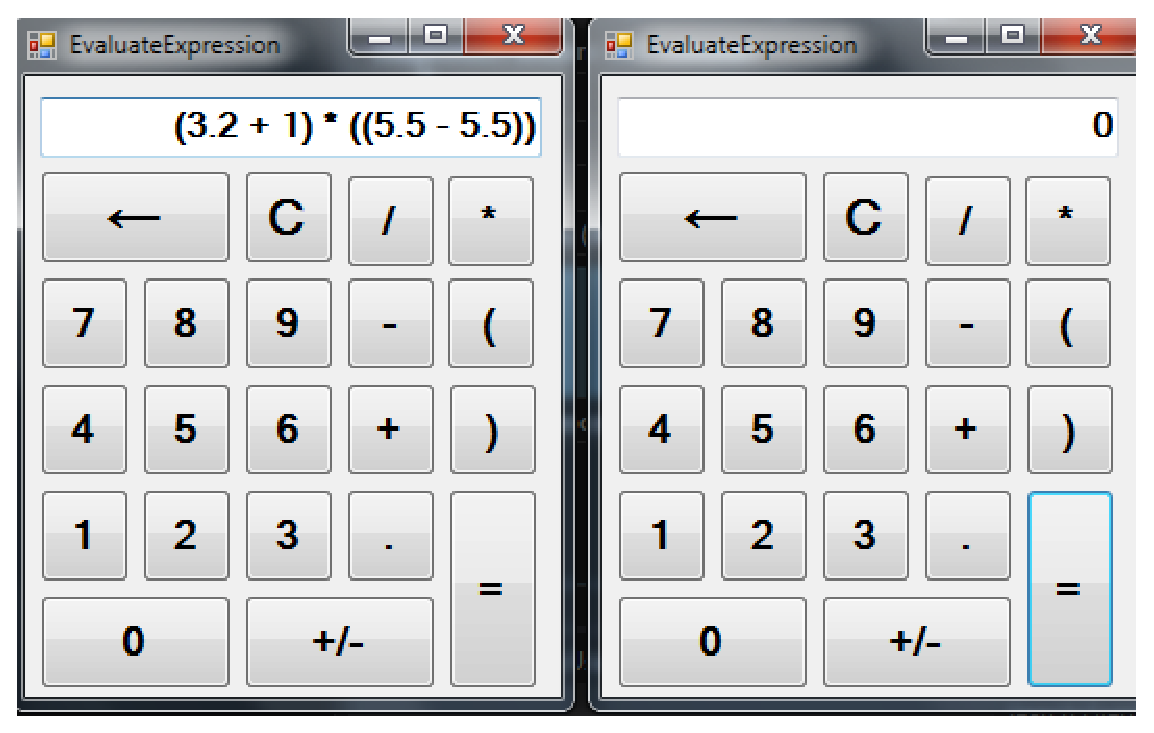
\includegraphics[width=\textwidth]{7.eps}\\

\cleardoublepage
\section*{Concluzie}
\phantomsection

\tab In lucrarea data am creat 2 versiuni de calculatoare. Fiecare calculator
avind specificul sau si constructia sa. Am invatat sa "impachetam" programele
noastre intr-un mod mai prielnic unui User. Astfel putem crea aplicatii User
friendly. Spre deosebire de primul calculator, al doilea are separat
functionalitatea sa in alte fisiere si algoritmul de rezolvare ramine acelasi.
In urma efectuarii lucrarii mi-am imbogatit cunostintele in ceea ce priveste crearea aplicatiilor GUI. Acum putem sa nu folosim mereu consola dar sa comunicam
cu programul nostru printr-o forma mai placuta si mai familiara unui simplu
utilizator. Drept IDE am ales \textbf{Visual Studio} din cauza ca am gasit mai multa
informatie despre el. Am utilizat limbajul \textbf{C++} iar partea functionala
e scrisa in \textbf{C}. Un avantaj foarte mare a unui mediu interactiv este
faptul ca ne permite sa cream un lucru intr-un timp foarte scurt si totodata
sa evitam multe greseli. Dupa parerea mea lucrarea data este foarte importanta
pentru un student TI, personal am acumulat multe cunostinte noi in urma
efectuarii acesteia.
\end{document}
